%
% Der Satz von Gauss in Dimension n=3
%
\section{Der Satz von Gauss in Dimension $n=3$
\label{buch:gauss:section:dimension3}}
\kopfrechts{Der Satz von Gauss in Dimension $n=3$}
Die Sätze von Green und Stokes haben gezeigt, wie sich das Verhalten
einer Ableitung im Inneren eines zweidimensionalen Gebietes oder
einer im Raum eingetteten Fläche aus den Werten auf dem Rand erschliessen
lässt.
Er verallgemeinert den Hauptsatz der Infinitesimalrechnung, der dieselbe
Art von Aussage für eindimensionale Gebiete oder In den Raum eingebettete
Kurven macht.
Es gibt aber keinen Grund, bei den Dimensionen 1 und 2 stehen zu bleiben.
In diesem Abschnitt wird der Fall $n-1=2$ und $n=3$ genauer untersucht,
der traditionell als der Satz von Gauss bekannt ist.
Im nächsten Abschnitt wird dies dann auf beliebige Dimension verallgemeinert.

Die Vorgehensweise ist völlig analog zum zweidimensionalen Fall.
Die Argumente werden daher teilweise nicht im gleichen Detail
wie in Kapitel~\ref{chapter:green} präsentiert.

%
% Integration auf dreidimensioinalen Mannigfaltigkeiten
%
\subsection{Integration auf dreidimensionalen Mannigfaltigkeiten}
Zunächst muss die Integration von zwei auf drei Dimensionen erweitert
werden.
Dabei tauchen als natürliche Konstrukte die Begriff von 3-Vektor und
3-Form auf.

\subsubsection{Dreifache Integrale}
Sei $f\colon U\to\mathbb{R}:(x,y,z)\mapsto f(x,y,z)$ eine
stetige Funktion, die in einer offenen Teilmenge $U\subset\mathbb{R}^3$
definiert ist.
Wir betrachten ein Gebiet $V\subset U$, welches
durch die Ungleichungen
\[
x_-\le x \le x_+,
\qquad
y_-(x)\le y\le y_+(x)
\qquad\text{und}\qquad
z_-(x,y)\le z\le z_+(x,y)
\]
beschrieben werden kann, wobei die Funktionen $y_{\pm}$ und $z_{\pm}$
ebenfalls stetig sein sollen.

Das (dreifache) Integral der Funktion $f$ über die Menge $V$ ist dann durch 
das iterierte Integral
\begin{align}
\underset{V}{\int\!\!\!\int\!\!\!\int}
f(x,y,z)\,dx\,dy\,z
&=
\int_{x_-}^{x_+}
\int_{y_-(x)}^{y_+(x)}
\int_{z_-(x,y)}^{z_+(x,y)}
f(x,y,z)
\,dz
\,dy
\,dx
\label{buch:gauss:3d:eqn:integral}
\end{align}
gegeben.
Der Satz von Fubini besagt, dass eine alternative Beschreibung des
Gebietes zum Beispiel durch Ungleichungen der Form
\[
y_-\le y \le y_+,
\qquad
z_-(y)\le z\le z_+(y)
\qquad\text{und}\qquad
x_-(y,z)\le x\le x_+(y,z)
\]
auf den gleichen Wert
\begin{align*}
\underset{V}{\int\!\!\!\int\!\!\!\int}
f(x,y,z)\,dx\,dy\,z
&=
\int_{y_-}^{y_+}
\int_{z_-(y)}^{z_+(y)}
\int_{x_-(y,z)}^{x_+(y,z)}
f(x,y,z)
\,dx
\,dz
\,dy
\end{align*}
führt.

%
% Volumenelement
%
\subsubsection{Volumenelement}
Der Ausdruck $dx\,dy\,dz$ in \eqref{buch:gauss:3d:eqn:integral}
wird auch als das Volumenelement in kartesischen Koordinaten bezeichnet.
Man stellt sich das Gebiet $V$ zusammengesetzt aus kleinen Quadern
an der Stelle $(x_i,y_i,z_i)$, $i=1,\dots,N$,
mit Seitenlängen $\Delta x$, $\Delta y$ und $\Delta z$, die ein
Volumen $\Delta x\,\Delta y\,\Delta z$ haben.
Dann bildet man riemannsche Summen
\[
I_N
=
\sum_{i=1}^N
f(x_i,y_i,z_i)\,\Delta x\,\Delta y\,\Delta z
\]
und lässt dann $N\to\infty$ gehen, wobei gleichzeitig die Kantenlängen
der Quader gegen Null gehen sollen.
Der Grenzwert
\[
\lim_{N\to\infty} I_N
=:
\underset{V}{\int\!\!\!\int\!\!\!\int}
f(x,y,z)\,dx\,dy\,z
\]
heisst, sofern er existiert, das Riemannsche Integral der Funktion $f$
über $V$.

%
% Koordinatenwechsel
%
\subsubsection{Koordinatenwechsel}
Wir betrachten jetzt die Wirkung eines Koordinatenwechsels.
Um die Notation etwas leichter nachvollziehbar zu gestalten, schreiben
wir die Koordinaten wieder in Indexnotation.
Die glatten Funktionen
\begin{equation}
y^i
=
y^i(x^1,x^2,x^3),\quad i\in\{1,2,3\}
\label{buch:gauss:3d:eqn:koordinatenabbildung}
\end{equation}
beschreiben den Wechsel der Koordinaten.

Das Volumenelement in den $x$-Koordinaten entsteht aus der Vorstellung
von kleinen Quadern mit Seitenkanten der Länge
$\Delta x^1$, 
$\Delta x^2$ und
$\Delta x^3$.
Die Kanten können durch die Standardbasisvektoren $\vec{e}_i$ als
$\vec{e}_1\Delta x^1$, $\vec{e}_2\Delta x^2$ und $\vec{e}_e\Delta x^3$
dargestellt werden.

Die Koordinatenabbildung~\eqref{buch:gauss:3d:eqn:koordinatenabbildung}
deformiert den Quader zu Körper mit gekrümmten Seitenkanten.
Für genügend kleine $\Delta x^i$ kann er approximiert werden durch
ein Parallelepiped mit den Seitenkante
\[
Dy\cdot(\vec{e}_i\Delta x^i)
=
\Delta x^i
\frac{\partial(y^1,y^2,y^3)}{\partial(x^1,x^2,x^3)}
\vec{e}_i
=
\Delta x^i
\renewcommand{\arraystretch}{2.0}
\begin{pmatrix}
\displaystyle\frac{\partial y^1}{\partial x^1}&
\displaystyle\frac{\partial y^1}{\partial x^2}&
\displaystyle\frac{\partial y^1}{\partial x^3}\\
\displaystyle\frac{\partial y^2}{\partial x^1}&
\displaystyle\frac{\partial y^2}{\partial x^2}&
\displaystyle\frac{\partial y^2}{\partial x^3}\\
\displaystyle\frac{\partial y^3}{\partial x^1}&
\displaystyle\frac{\partial y^3}{\partial x^2}&
\displaystyle\frac{\partial y^3}{\partial x^3}
\end{pmatrix}
\vec{e}_i
=
\Delta x^i
\begin{pmatrix}
\displaystyle\frac{\partial y^1}{\partial x^i}\\
\displaystyle\frac{\partial y^2}{\partial x^i}\\
\displaystyle\frac{\partial y^3}{\partial x^i}\\
\end{pmatrix}
\]
Die Funktionalmatrix $Dy$ bildet die Kantenvektoren ab.

Das Volumen des von den Vektoren $Dy\cdot\vec{e}_i$ aufgespannten
Parallelepipeds wird durch die Determinaten $\det Dy$ der
Abbildungsmatrix gegeben. 
Ist die Funktion $f$ in $y$-Koordinaten als $f(y^1,y^2,y^3)$ gegeben 
ist das Integral von $f$ daher 
\begin{align*}
\int\!\!\!\int\!\!\!\int
\tilde{f}(y_1,y_2,y_3)
\,dy^1
\,dy^2
\,dy^3
&=
\int\!\!\!\int\!\!\!\int
f(x^1,x^2,x^3)
\left|
\frac{\partial (y^1,y^2,y^3)}{\partial(x^1,x^2,x^3)}
\right|
\,dx^1
\,dx^2
\,dx^3.
\\
&=
\int\!\!\!\int\!\!\!\int
f(x^1,x^2,x^3)
\det Dy(x^1,x^2,x^3)
\,dx^1
\,dx^2
\,dx^3.
\end{align*}
Das Integral einer Funktion ist also nicht koordinatenunabhängig:

%
% 3-Vektoren
%
\subsubsection{3-Vektoren}
In Abschnitt~\ref{buch:green:section:integral} wurde dargestellt, wie
das Integral einer 2-Form definiert werden kann.
Dabei wurde ausführlich erklärt, wie eine 2-Form die richtigen
Transformationseigenschaften hat, damit das Integral der 2-Form
eine koordinatenaunabhängige Grösse wird.
Wir übertragen daher die Definition von 2-Fektoren und 2-Formen
auf den dreidimensionalen Fall.

Ein 3-Vektor ist eine Linearkombination von Tensoren dritter Stufe
Die drei Faktoren müssen vollständig antisymmetrisch sein.
Jede Vertauschung muss das Vorzeichen kehren.
Dies führt auf die komplizierte Summe
\begin{align}
\vec{e}_i
\wedge
\vec{e}_k
\wedge
\vec{e}_l
&=
\phantom{+}
\vec{e}_i\otimes\vec{e}_k\otimes\vec{e}_l
+
\vec{e}_k\otimes\vec{e}_l\otimes\vec{e}_i
+
\vec{e}_l\otimes\vec{e}_i\otimes\vec{e}_k
\\
&\phantom{=}
-
\vec{e}_i\otimes\vec{e}_l\otimes\vec{e}_k
-
\vec{e}_l\otimes\vec{e}_k\otimes\vec{e}_i
-
\vec{e}_k\otimes\vec{e}_i\otimes\vec{e}_l.
\label{buch:gauss:3d:eqn:3vektor}
\end{align}
Um solche Ausdrücke einfacher schreiben zu können führen wir das
Levi-Cività-Symbol ein.
Dazu brauchen wir zunächst den Begriff der geraden bzw.~ungeraden
Permutation.

\begin{definition}[Gerade und ungerade Permutation]
Eine Permutation $i_1,\dots,i_n$ der Zahlen $1,\dots,n$ heisst {\em gerade},
wenn sie durch eine gerade Anzahl Vertauschungen von aus $1,\dots,n$
entsteht.
Sie heisst {\em ungerade}, wenn eine ungerade Anzahl Vertauschungen
nötig ist
\index{gerade Permutation}%
\index{ungerade Permutation}%
\end{definition}

Für $n=2$ sind $(1,2)$ und $(2,1)$ die einzigen Permutationen,
die erste ist gerade, die zweite ungerade.
Für $n=3$ gibt es insgesamt 6 Permutationen, nämlich
\[
\begin{aligned}
&\text{gerade:}  &&(1,2,3),\;(2,3,1),\;(3,1,2)\\
&\text{ungerade:}&&(1,3,2),\;(3,2,1),\;(2,1,3).
\end{aligned}
\]
Für die Formel \eqref{buch:gauss:3d:eqn:3vektor} ist vor allem
das Vorzeichen der einzelnen Terme wichtig.
Das Levi-Cività-Symbol definiert dieses.

\begin{definition}[Levi-Cività-Symbol]
Das Levi-Cività-Symbol $n$-ter Stufe ist definiert durch
\[
\varepsilon_{i_1\dots i_n}
=
\begin{cases}
\phantom{-}1&\qquad\text{$i_1,\dots,i_n$ ist eine gerade Permutation}\\
         - 1&\qquad\text{$i_1,\dots,i_n$ ist eine ungerade Permutation}\\
\phantom{-}0&\qquad\text{sonst}
\end{cases}
\]
\end{definition}

Mit dem Levi-Cività-Symbol kann man 
\eqref{buch:gauss:3d:eqn:3vektor}
als
\[
\vec{e}_1
\wedge
\vec{e}_2
\wedge
\vec{e}_3
=
\sum_{i_1,\dots,i_n=1}^n
\varepsilon_{i_1 i_2 i_3}
\vec{e}_{i_1}
\otimes
\vec{e}_{i_2}
\otimes
\vec{e}_{i_3}
\]
schreiben.
Für Tensorfelder auf einer Mannigfaltigkeit kann auch die Schreibweise
\[
\frac{\partial}{\partial x^1}
\wedge
\frac{\partial}{\partial x^1}
\wedge
\frac{\partial}{\partial x^1}
=
\sum_{i_1,\dots,i_3=1}^3
\varepsilon_{i_1 i_2 i_3}
\frac{\partial}{\partial x^{i_1}}
\otimes
\frac{\partial}{\partial x^{i_2}}
\otimes
\frac{\partial}{\partial x^{i_3}}
\]
verwendet werden.
So wie es in zwei Dimensionen der Raum der 2-Vektoren eindimensional
war, ist in drei Dimensionen der Raum der 3-Vektoren eindimensional
und $\vec{e}_1\wedge\vec{e}_2\wedge\vec{e}_3$ kann als Basisvektor
betrachtet werden.

%
% 3-Formen
%
\subsubsection{3-Formen}
Dual zum Konzept des 3-Vektors können wir auch die 3-Formen
\[
\omega(x)
=
f(x)
dx^1 \wedge dx^2 \wedge dx^3
\]
auf der Mannigfaltigkeit betrachten.
Auch der Vektorraum der 3-Formen ist eindimensional.
Bei einem Koordinatenwechsel wird $f$ mit der Funktionaldeterminante
multipliziert.

%
% Integral einer 3-Form
%
\subsubsection{Integral einer 3-Form}
Zu einer 3-Form $\omega(x)=f(x)\,dx^1\wedge dx^2\wedge dx^3$ können wir 
in Koordinaten das Integral über eine Karte $(V,\varphi)$
\[
\int_{V} \omega
=
\underset{\varphi(V)}{\displaystyle\int\!\!\!\int\!\!\!\int}
f(x^1,x^2,x^3)
\,
dx^1\,dx^2\,dx^3
\]
definieren.
Da bei einem Koordinatenwechsel die 3-Form mit der Funktionaldeterminante
multipliziert wird, ist das Integral unabhängig vom gewählten
Koorinatensystem.

%
% Der Satz von Gauss
%
\subsection{Der Satz von Gauss}
%
% fig-gaussrand.tex
%
% (c) 2025 Prof Dr Andreas Müller
%
\begin{figure}
\centering
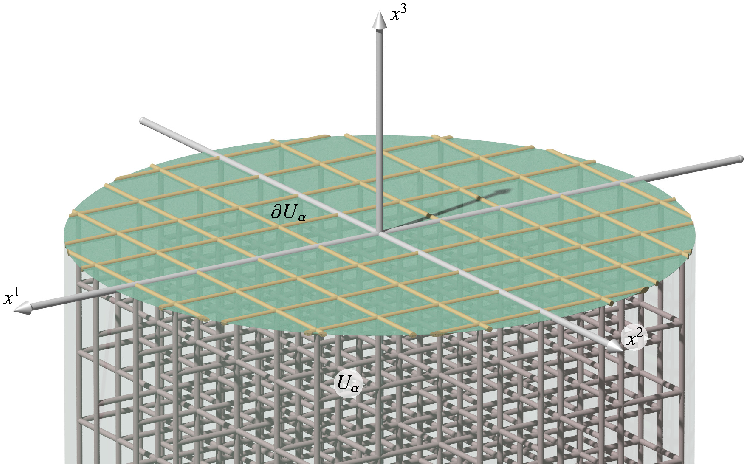
\includegraphics[width=\textwidth]{chapters/050-gauss/images/gaussrand.pdf}
\caption{Rand $\partial U_\alpha$ einer Karte $U_\alpha$ einer
dreidimensionalen Mannigfaltigkeit mit Rand für die Herleitung des
Satzes von Gauss.
\label{buch:gauss:fig:gaussrand}}
\end{figure}

Die zentrale Idee im Satz von Green war, dass sich das Integral
der Ableitung einer Funktion in Richtung senkrecht sofort auswerten
lässt.
Es blieb dann ein Integral über den Rand.
Die gleiche Argumentation funktioniert auch in drei Dimensionen.

%
% Integral und Rand
%
\subsubsection{Integral und Rand}
Sei $f\colon\mathbb{R}^2\times\mathbb{R}_{\le 0}\to \mathbb{R}$
eine Funktion mit kompaktem Träger
(Abbildung~\ref{buch:gauss:fig:gaussrand}).
Das Integral der 3-Form
\[
\omega
=
\frac{\partial f}{\partial x^3}(x^1,x^2,x^3)\,dx^1\wedge dx^2\wedge dx^3
\]
ist dann
\begin{align*}
\int_V
\frac{\partial f}{\partial x^3}(x^1,x^2,x^3)\,dx^1\wedge dx^2\wedge dx^3
&=
\int_{-\infty}^0
\int_{-\infty}^{\infty}
\int_{-\infty}^{\infty}
\frac{\partial f}{\partial x^3}(x^1,x^2,x^3)
\,dx^1
\,dx^2
\,dx^3.
\intertext{Die Integrationen dürfen vertaiuscht werden, das Integral
wird dann zu}
&=
\int_{-\infty}^{\infty}
\int_{-\infty}^{\infty}
\int_{-\infty}^0
\frac{\partial f}{\partial x^3}(x^1,x^2,x^3)
\,dx^3
\,dx^1
\,dx^2
\\
&=
\int_{-\infty}^{\infty}
\int_{-\infty}^{\infty}
\Bigl[
f(x^1,x^2,x^3)
\Bigl]_{x^3=-\infty}^{x^3=0}
\,dx^1
\,dx^2
\\
&=
\int_{-\infty}^{\infty}
\int_{-\infty}^{\infty}
f(x^1,x^2,0)
\,dx^1
\,dx^2
\\
&=
\int_{\partial V} f(x^1,x^2,0) \,dx^1\wedge dx^2.
\end{align*}
Das verbleibende Integral ist also ein Integral der Funktion $f$
über den Rand.

Eine einzelne partielle Ableitung kann natürlich keine
koordinatenunabhängige Eigenschaft sein.
In drei Dimensionen gibt es drei mögliche partielle Ableitungen.
Wie im Fall des Satzes von Green kombinieren wir daher 
drei partielle Ableitungen zur 3-Form
\begin{equation}
\omega
=
\biggl(
\frac{\partial f_{23}}{\partial x^1}
+
\frac{\partial f_{13}}{\partial x^2}
+
\frac{\partial f_{12}}{\partial x^3}
\biggr)
\,dx^1\wedge dx^2\wedge dx^3.
\label{buch:gauss:3d:eqn:divform}
\end{equation}
Jeder Summand kann integriert werden, es bleibt dann für jeden
Term ein Integral über eine 2-Form.
\begin{align}
\int_V \omega
&=
\int_{\partial V} f_{23} \,dx^2\wedge dx^3
-
\int_{\partial V} f_{13} \,dx^1\wedge dx^3
+
\int_{\partial V} f_{12} \,dx^1\wedge dx^2
\label{buch:gauss:3d:eqn:gaussvorstufe}
\end{align}
Das Vorzeichen im mittleren Term kommt von der Orientierung
der Seitenflächen.
%
% fig-oberflaeche.tex
%
% (c) 2025 Prof Dr Andreas Müller
%
\begin{figure}
\centering
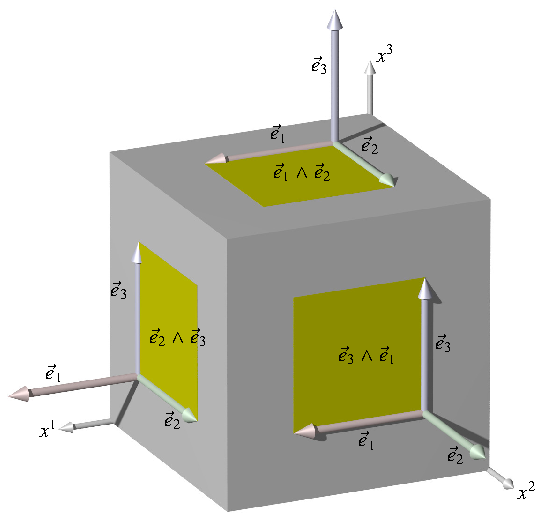
\includegraphics{chapters/050-gauss/images/oberflaeche.pdf}
\caption{Die Seitenflächen eines Koordinatenwürfels werden von den
Basis-2-Vektoren aufgespannt.
Für den Satz von Gauss müssen diese Seitenflächen untereinander kompatibel
orientiert sein.
Daher muss die von den Richtungen $\vec{e}_1$ und $\vec{e}_3$ aufgespannte
Seitenfläche die Orientierung von
$\vec{e}_3\wedge\vec{e}_1=-\vec{e_1}\wedge\vec{e_3}$
haben.
\label{buch:gauss:fig:oberflaeche}}
\end{figure}
%
In Abbildung~\ref{buch:gauss:fig:oberflaeche} sind die
2-Vektoren dargestellt, die die Seitenflächen eines achsparallelen
Würfels aufspannen.
Damit alle Seitenflächen die gleiche Orientierung verwenden, muss
die Seitenfläche senkrecht auf die $x^2$-Richtung den 2-Vektor
$\vec{e}_3\wedge\vec{e}_1=-\vec{e}_1\wedge\vec{e}_3$
verwenden.

%
% Äussere Ableitung einer 2-Form
%
\subsubsection{Äussere Ableitung einer 2-Form}
Der Ausdruck \eqref{buch:gauss:3d:eqn:divform} hat einige Ähnlichkeit
zur 2-Form, die durch äussere Ableitung einer 1-Form entsteht.
Wir definieren daher die äussere Ableitung der 2-Form
\[
\alpha
=
f_{12}(x) \,dx^1\wedge dx^2
+
f_{13}(x) \,dx^1\wedge dx^3
+
f_{23}(x) \,dx^2\wedge dx^3
\]
als
\begin{align*}
d\alpha
&=
\frac{\partial f_{12}}{\partial x^3} \,
dx^3\wedge dx^1\wedge dx^2
+
\frac{\partial f_{13}}{\partial x^2} \,
dx^2\wedge dx^1\wedge dx^3
+
\frac{\partial f_{23}}{\partial x^1} \,
dx^1\wedge dx^2\wedge dx^3.
\intertext{Durch Vertauschung der 1-Formen samt zugehörigen Vorzeichenwechseln
kann erreicht werden, dass alle Summanden Vielfache der gleichen
3-Form $dx^1\wedge dx^2\wedge dx^3$}
&=
\frac{\partial f_{12}}{\partial x^3} \,
dx^1\wedge dx^2 \wedge dx^3
-
\frac{\partial f_{13}}{\partial x^2} \,
dx^1\wedge dx^2\wedge dx^3
+
\frac{\partial f_{23}}{\partial x^1} \,
dx^1\wedge dx^2\wedge dx^3
\\
&=
\biggl(
\frac{\partial f_{23}}{\partial x^1}
-
\frac{\partial f_{13}}{\partial x^2}
+
\frac{\partial f_{12}}{\partial x^3}
\biggr)
\,dx^1\wedge dx^2\wedge dx^3.
\end{align*}
sind.

%
% Der Satz von Gauss
%
\subsubsection{Der Satz von Gauss}
Mit der äusseren Ableitung kann jetzt die
Integralbeziehung \eqref{buch:gauss:3d:eqn:gaussvorstufe}
in der Form des folgenden Satzes geschrieben werden.

\begin{satz}[Gauss]
Sie $\alpha$ eine 2-Form auf einer 3-dimensionalen Mannigfaltigkeit
$V$ mit Rand $\partial V$.
Dann gilt
\begin{equation}
\int_V d\alpha = \int_{\partial V}\alpha.
\label{buch:gauss:3d:satz:gauss:eqn}
\end{equation}
\end{satz}

Rein formal hat der Satz von Gauss die gleiche Form wie der
Satz von Stokes~\ref{buch:green:green:satz:stokes}.
Da auch der Beweis genau nah dem gleichen Muster erfolgt,
kann man vermuten, dass sich die Begriffe der $p$-Formen, der
äusseren Ableitung und des Integrals einer $p$-Form auf
beliebige Dimensionen verallgemeinern lässt.
Dies wird später in Kapitel~\ref{chapter:pformen} durchgeführt.

%
% Divergenz eines Vektorfeldes
%
\subsubsection{Divergenz eines Vektorfeldes}
In der klassischen Vektoranalysis wird die {\em Divergenz} eines Vektorfeldes
\index{Divergenz}%
$\vec{v}$ mit den Komponenten $v^i$, $i=1,\dots,3$, als
\[
\operatorname{div}\vec{v}
=
\frac{\partial v^1}{\partial x^1}
+
\frac{\partial v^2}{\partial x^2}
+
\frac{\partial v^3}{\partial x^3}
\in
\mathbb{R}.
\]
Das Integral 3-Form auf der linken Seite von
\eqref{buch:gauss:3d:satz:gauss:eqn}
im Satz von Gauss entspricht also einem Volumenintegral
der Divergenz.
Die rechte Seite von \eqref{buch:gauss:3d:satz:gauss:eqn}
ist ein Integral über eine Summe von Integranden der Form
$f_{ik}(x)\,dx^i\wedge dx^k$.
Die 2-Form $dx^i\wedge dx^k$ berechnet die Projektion eines
Parallelepipeds auf die Ebene aufgespannt von den Vektoren
$\vec{e}_i$ und $\vec{e}_k$.
Schreibt man $\vec{n}$ für die Normale eines Parallelepipeds
der Oberfläche von $V$, dann kann man den Integranden
auf der rechten Seite von \eqref{buch:gauss:3d:satz:gauss:eqn}
als das Skalarprodukt $\vec{v}\cdot d\vec{n}$ interpretieren.
In der klassischen Form wird der Satz von Gauss daher auch
in der Form
\[
\underset{V}{\int\!\!\!\int\!\!\!\int}
\operatorname{div}\vec{v}
\,dx\,dy\,dz
=
\int_{\partial V}\vec{v}\cdot d\vec{n}.
\]
geschrieben.

